\chapter[Resultados]{Resultados}
\label{result}

	Para cada \textit{shader} foram plotados os gráficos das métricas relacionadas ao \textit{vertex} e ao \textit{fragment shaders} e de todo o processo de renderização para diferentes dispositivos. Após as plotagens, percebeu-se que para todos os \textit{shaders} de todos os dispositivos, todos os gráficos relacionados ao \textit{vertex shader} possuíam curvas semelhantes. O mesmo ocorreu para o \textit{fragment shader} e para todo o processo de renderização.

\section{Dispositivos \textit{Android}} 

	Com o dispositivo \textit{Nexus 4} foi possível plotar os gráficos tanto para todo o processo de renderização, quanto para o \textit{vertex} e \textit{fragment shaders}. Assim, foi visto que os gráficos de todos os \textit{shaders} relacionados ao vértice resultaram em uma função linear (diferindo na inclinação)  e os relacionados ao fragmento e todo o processo de renderização deram curvas de formato semelhantes, embora não fosse possível determinar a curva exatamente apenas pela inspeção visual.  A Figura \ref{nexus1} e a Figura \ref{nexus2} mostram os gráficos plotados, com relação ao \textit{vertex} e \textit{fragment shaders} de cada \textit{shader} implementado, que demonstram a semelhança destas curvas. A Figura \ref{nexus3} também mostra esta semelhança para todo o processo de renderização de todos os \textit{shaders}.

	\begin{figure}[hb]
	\centering
		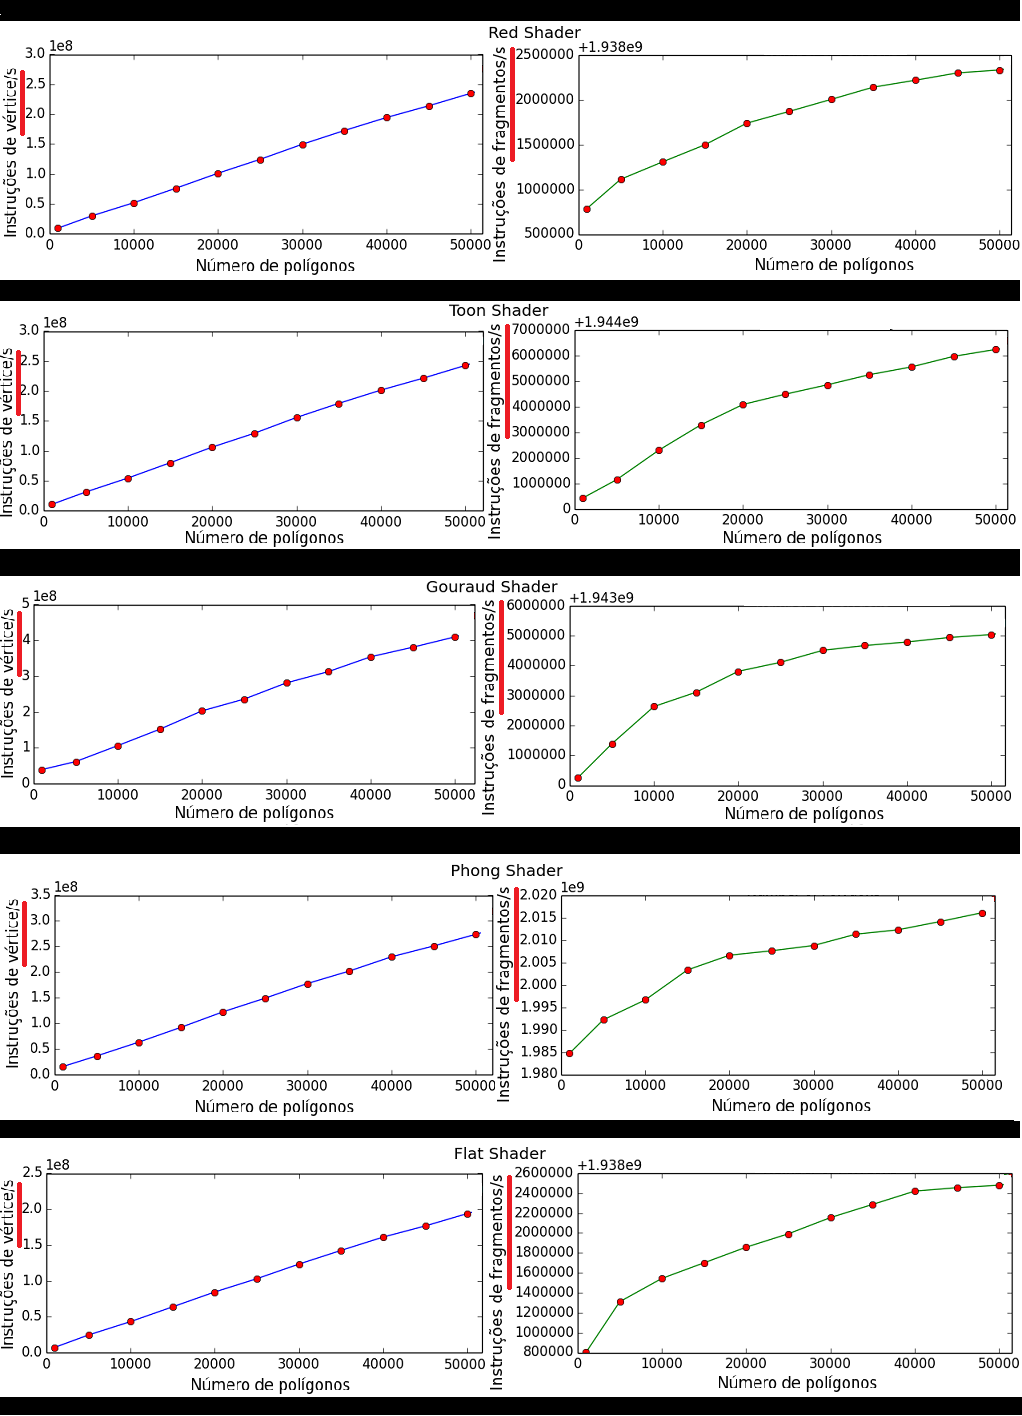
\includegraphics[keepaspectratio=true,scale=0.55]{figuras/red_pt.png}
	\caption{Gráficos: \textit{Red Shader}, \textit{Toon shader}, \textit{Gouraud Shader},  \textit{Phong Shader} e  \textit{Flat Shader} para o \textit{Nexus 4}}
	\label{nexus1}
	\end{figure}

	\begin{figure}[ht]
	\centering
		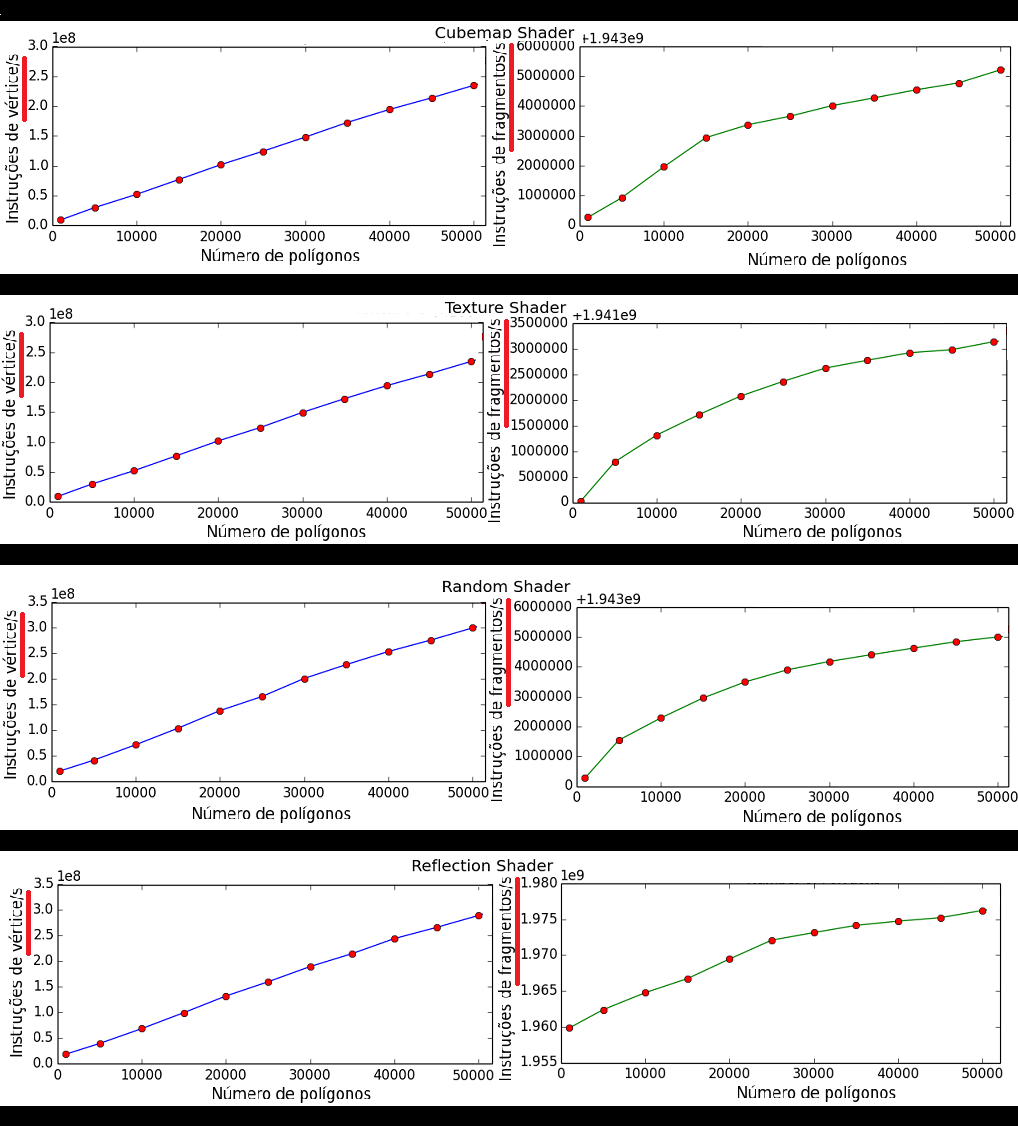
\includegraphics[keepaspectratio=true,scale=0.55]{figuras/cubeplot_pt.png}
	\caption{Gráficos: \textit{Cubemap Shader}, \textit{Texture Shader}, \textit{Random Shader}, \textit{Reflection Shader} para o \textit{Nexus 4}}
	\label{nexus2}
	\end{figure}

	\begin{figure}[ht]
	\centering
		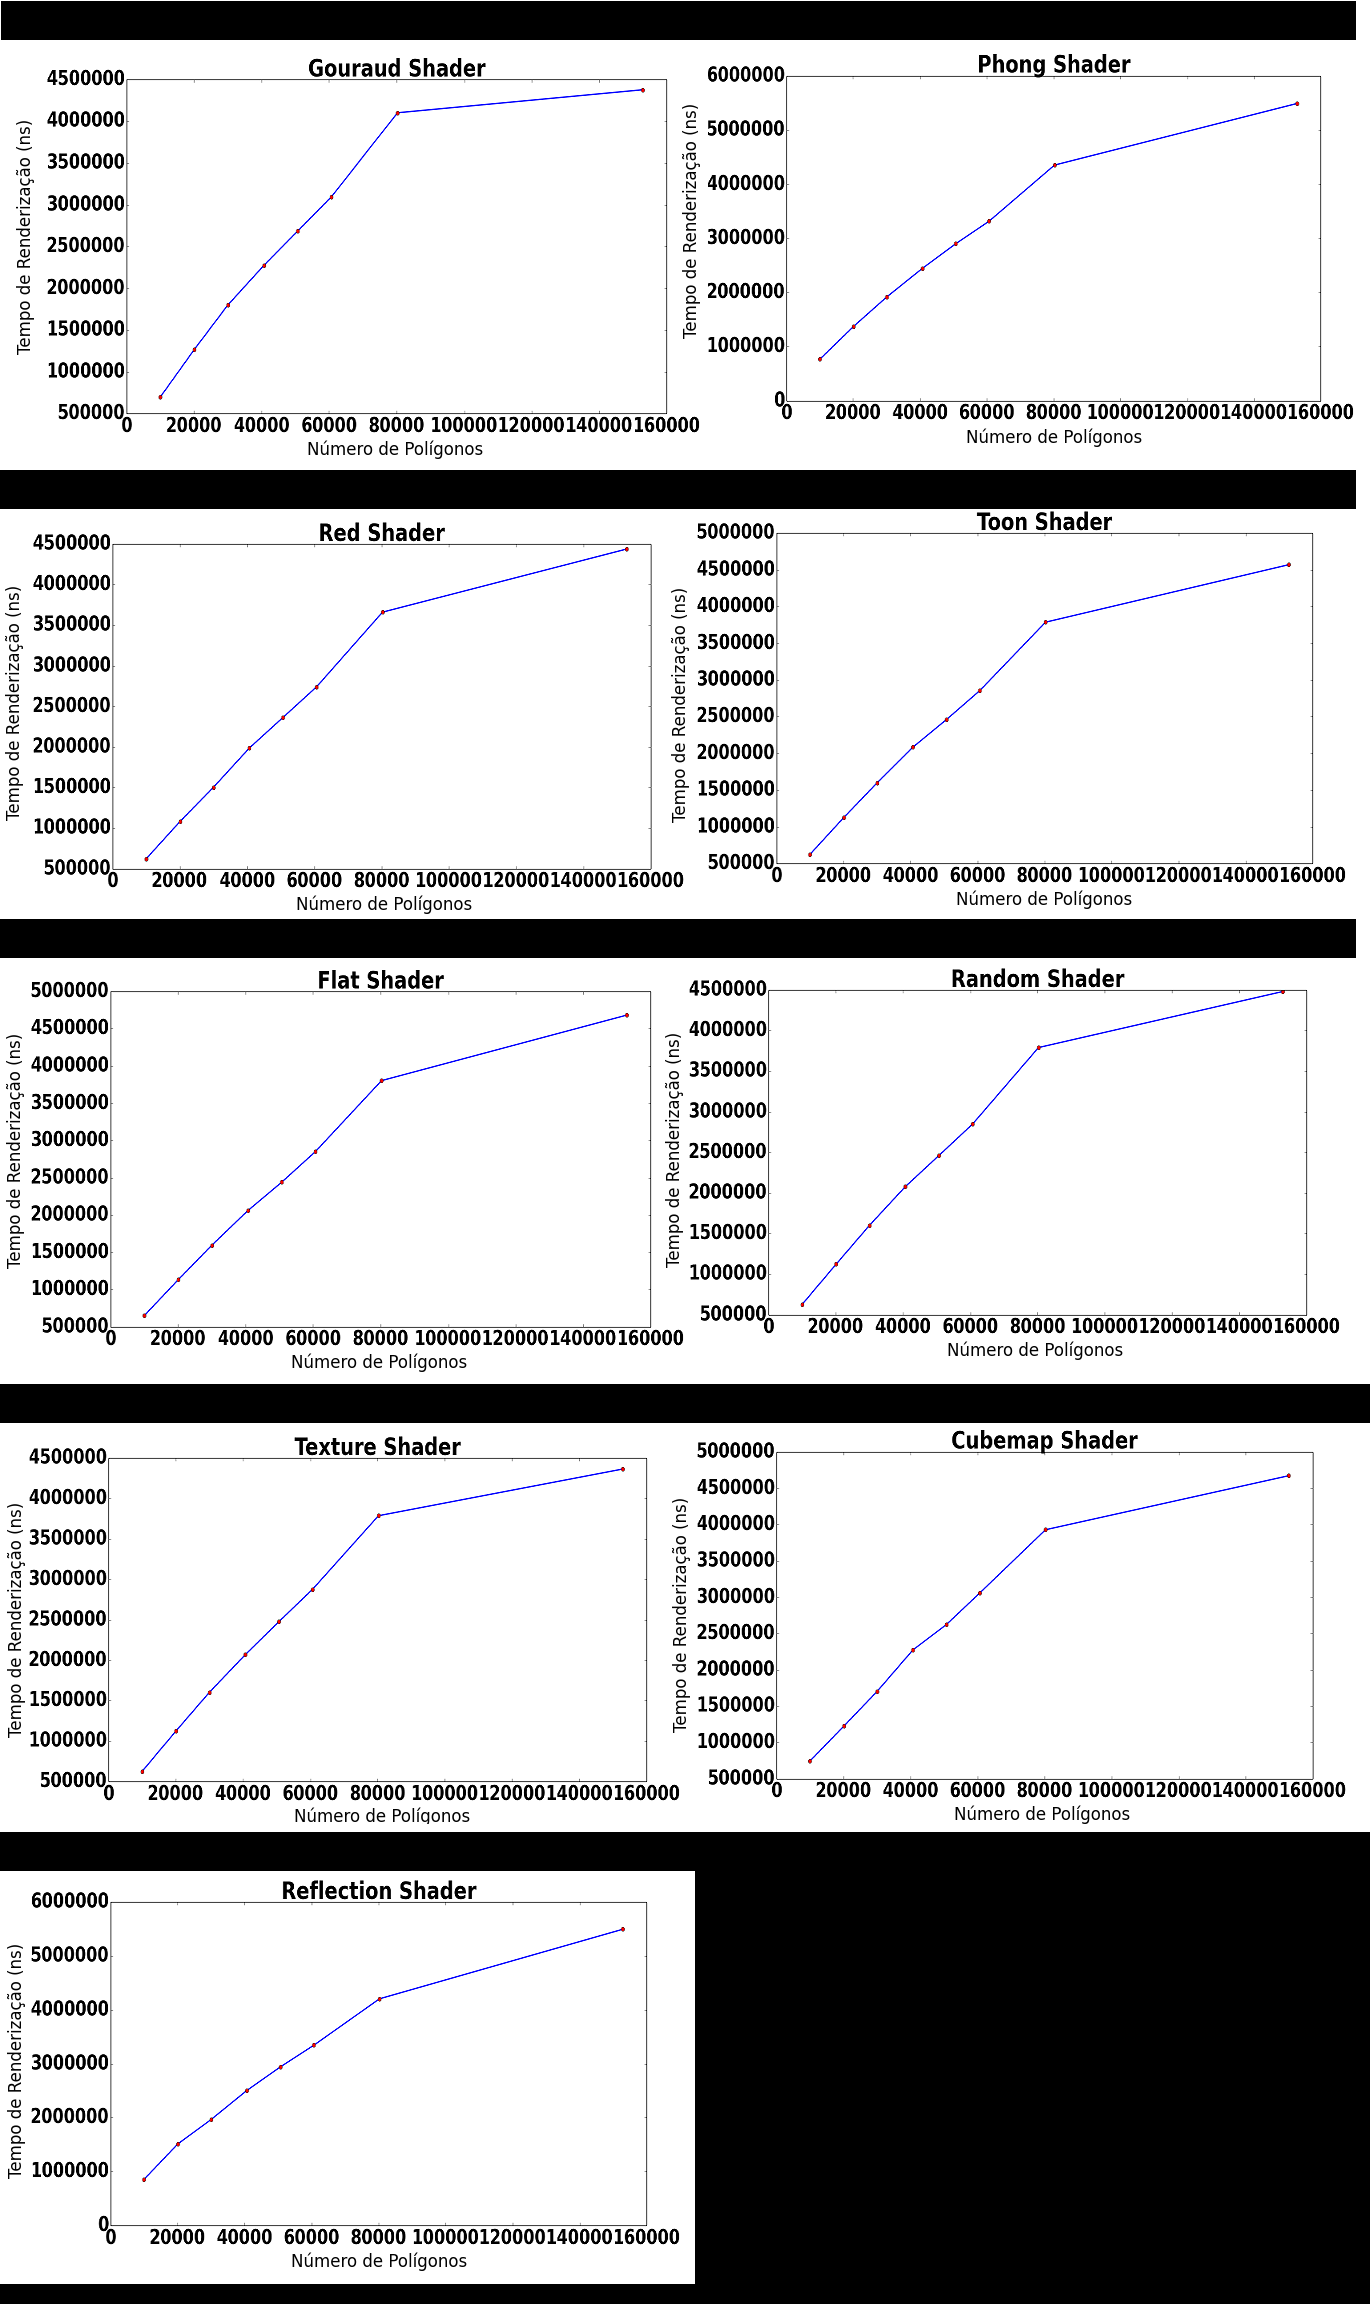
\includegraphics[keepaspectratio=true,scale=0.35]{figuras/render_time_pt.png}
	\caption{Gráficos relacionados ao tempo de renderização em nanosegundos para o \textit{Nexus 4}}
	\label{nexus3}
	\end{figure}	

	 A Figura \ref{comp_shaders2} e a Figura \ref{comp_shaders} faz uma comparação entre \textit{shaders}, em que todos os \textit{vertex e fragment shaders} são plotados em um mesmo gráfico, assim como as curvas relacionadas a todo o processo de renderização.	

	\begin{figure}[ht]
	\centering
		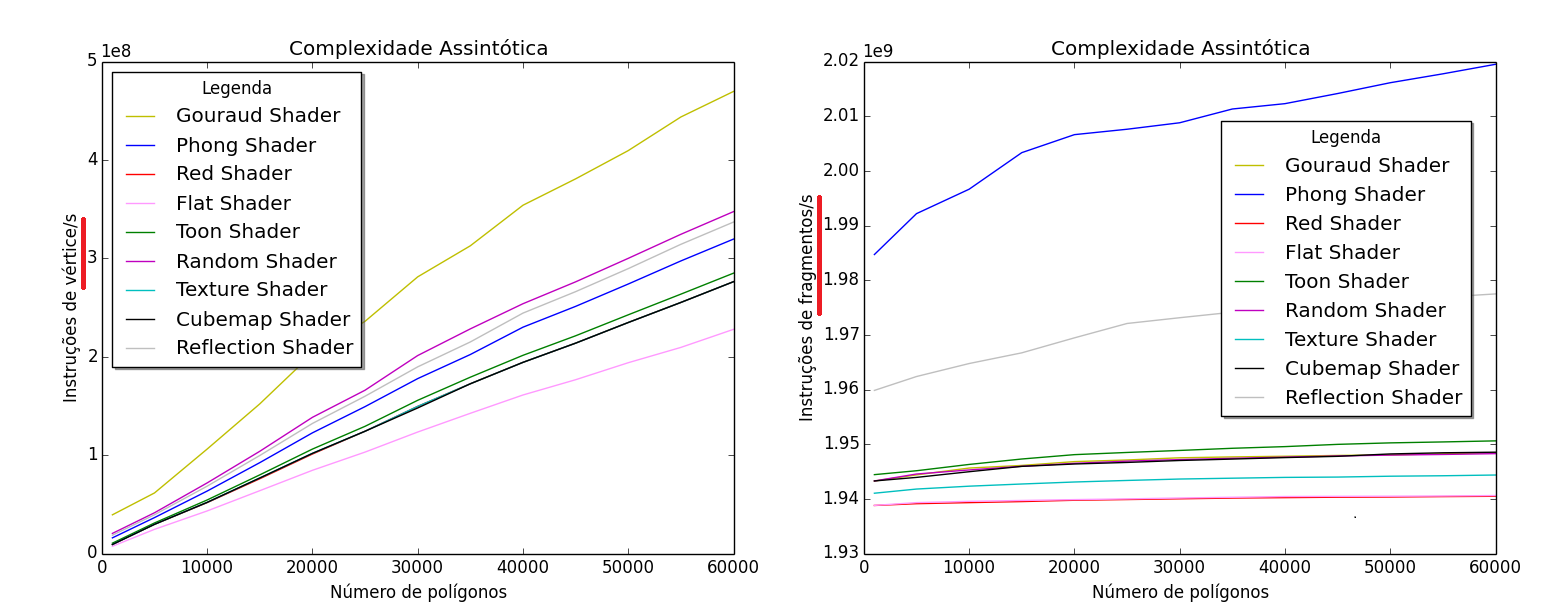
\includegraphics[keepaspectratio=true,scale=0.4]{figuras/devices_all.png}
	\caption{Comparações entre as curvas dos \textit{shaders}: todo processo de renderização}
	\label{comp_shaders2}
	\end{figure}	

	\begin{figure}[ht]
	\centering
		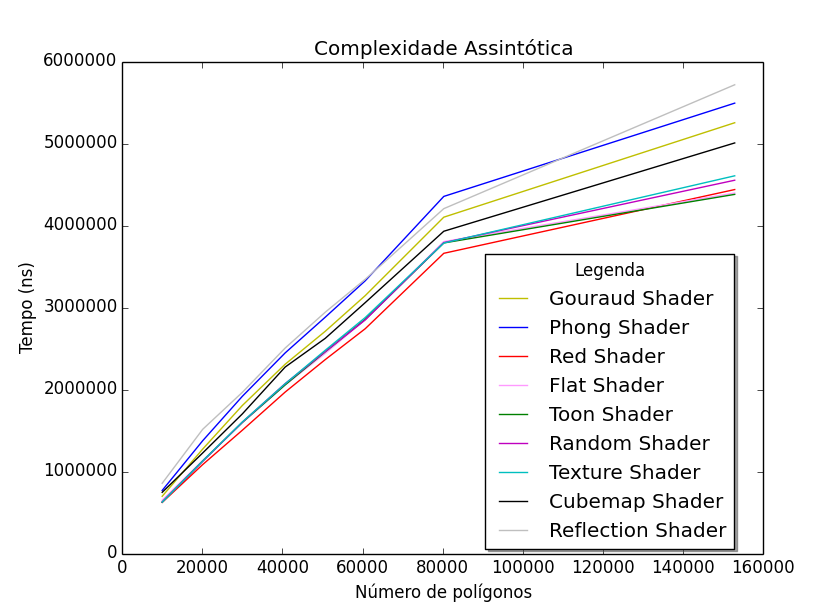
\includegraphics[keepaspectratio=true,scale=0.5]{figuras/render_time_all.png}
	\caption{Comparações entre as curvas dos \textit{shaders}: \textit{vertex} e \textit{fragment shaders}}
	\label{comp_shaders}
	\end{figure}	


	 Assim, os ajustes destas curvas desconhecidas em relação às curvas pré-definidas (linear, exponencial, polinômios de segundo e terceiro graus) também foram calculados e plotados para cada \textit{shader} (Figura \ref{nexus1_ajuste} e Figura \ref{nexus2_ajuste}, referentes ao \textit{Reflection Shader}). Também foram determinados os menores erros associados, a fim de descobrir qual curva melhor se ajustava às medições do \textit{fragment shader} e de todo o processo de renderização. Pela a análise do menor erro, calculado de acordo com a Seção \ref{metminqua}, todos os \textit{shaders} se aproximaram melhor de uma curva de terceiro grau, tanto para o \textit{fragment shader}, quanto para todo o processo de renderização.
	
	\begin{figure}[ht]
	\centering
		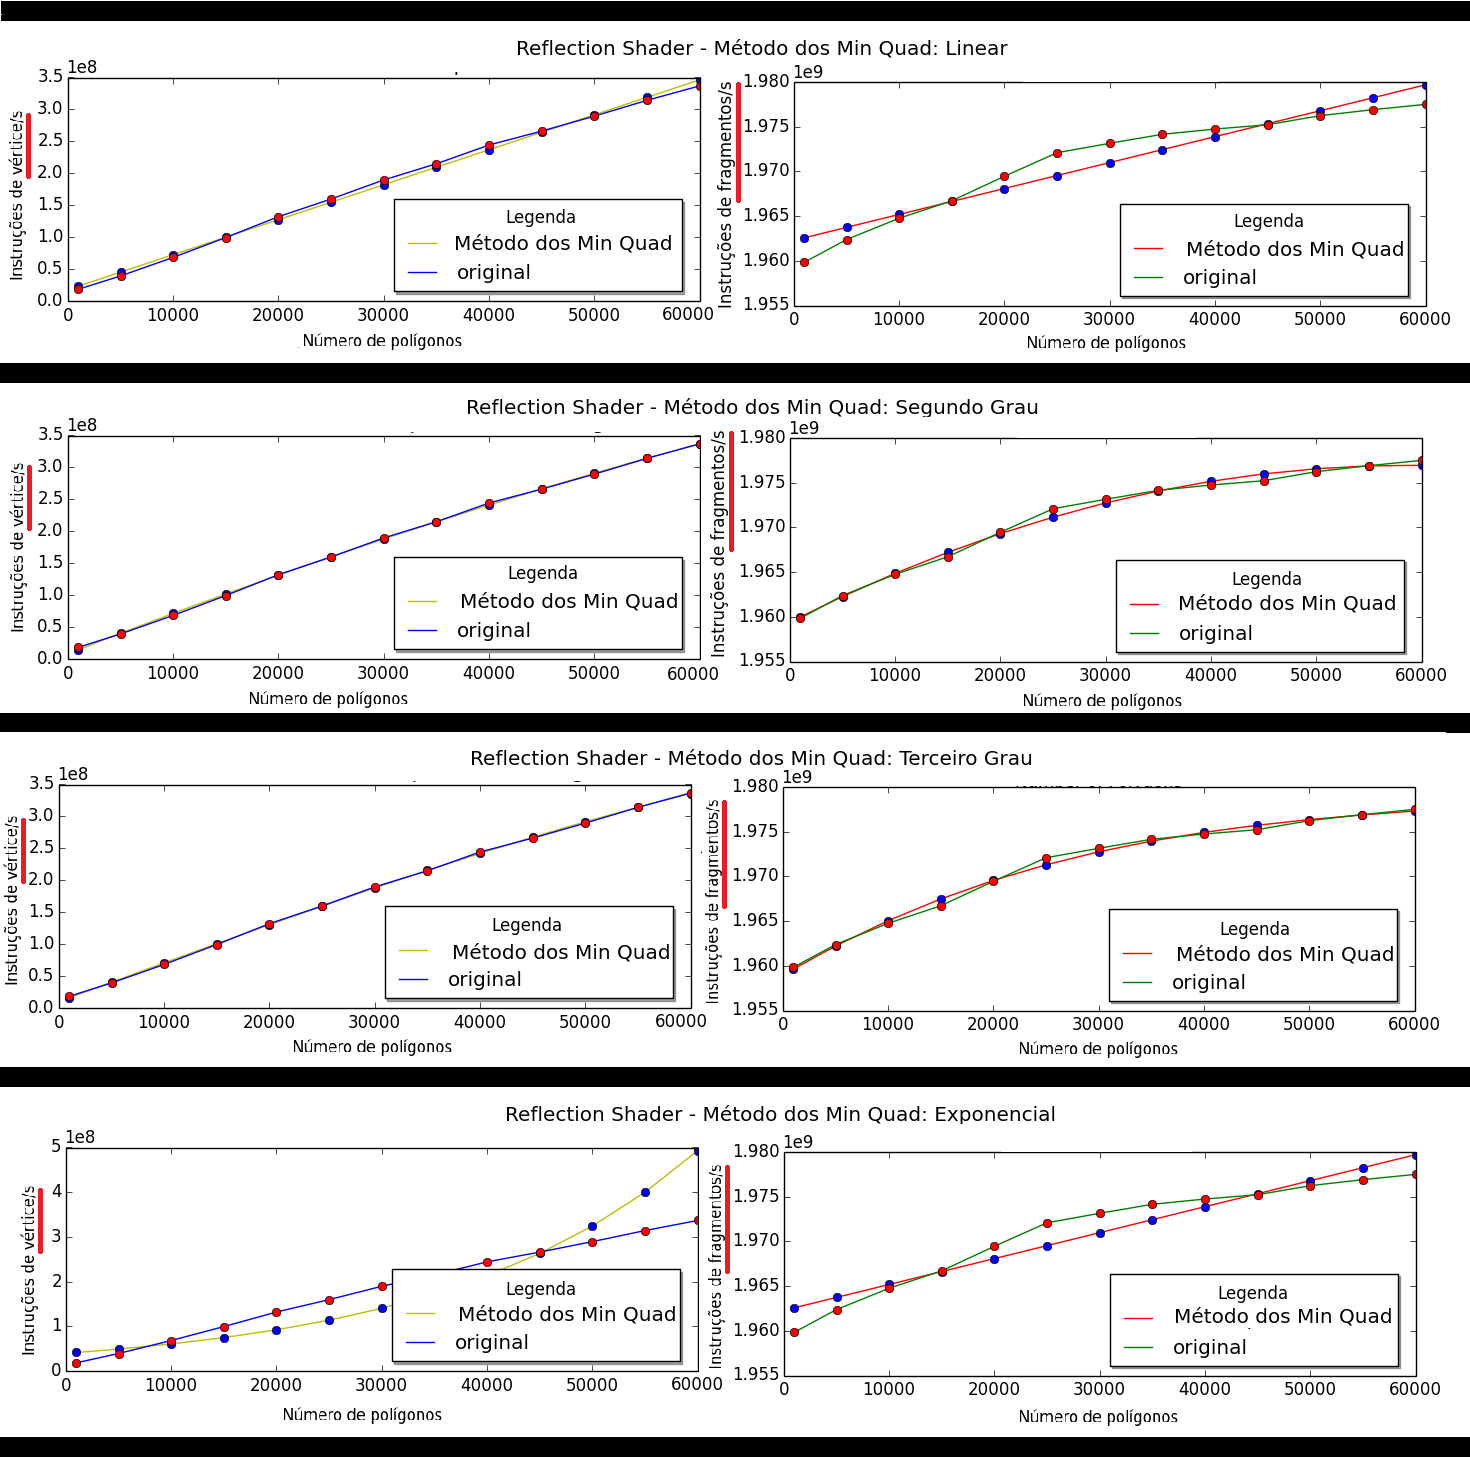
\includegraphics[keepaspectratio=true,scale=0.4]{figuras/reflectionlinear_pt.png}
	\caption{Ajustes linear, segundo, terceiro graus e exponencial de cada tipo de \textit{shader} para o \textit{Nexus 4}}
	\label{nexus1_ajuste}
	\end{figure}	

	\begin{figure}[ht]
	\centering
		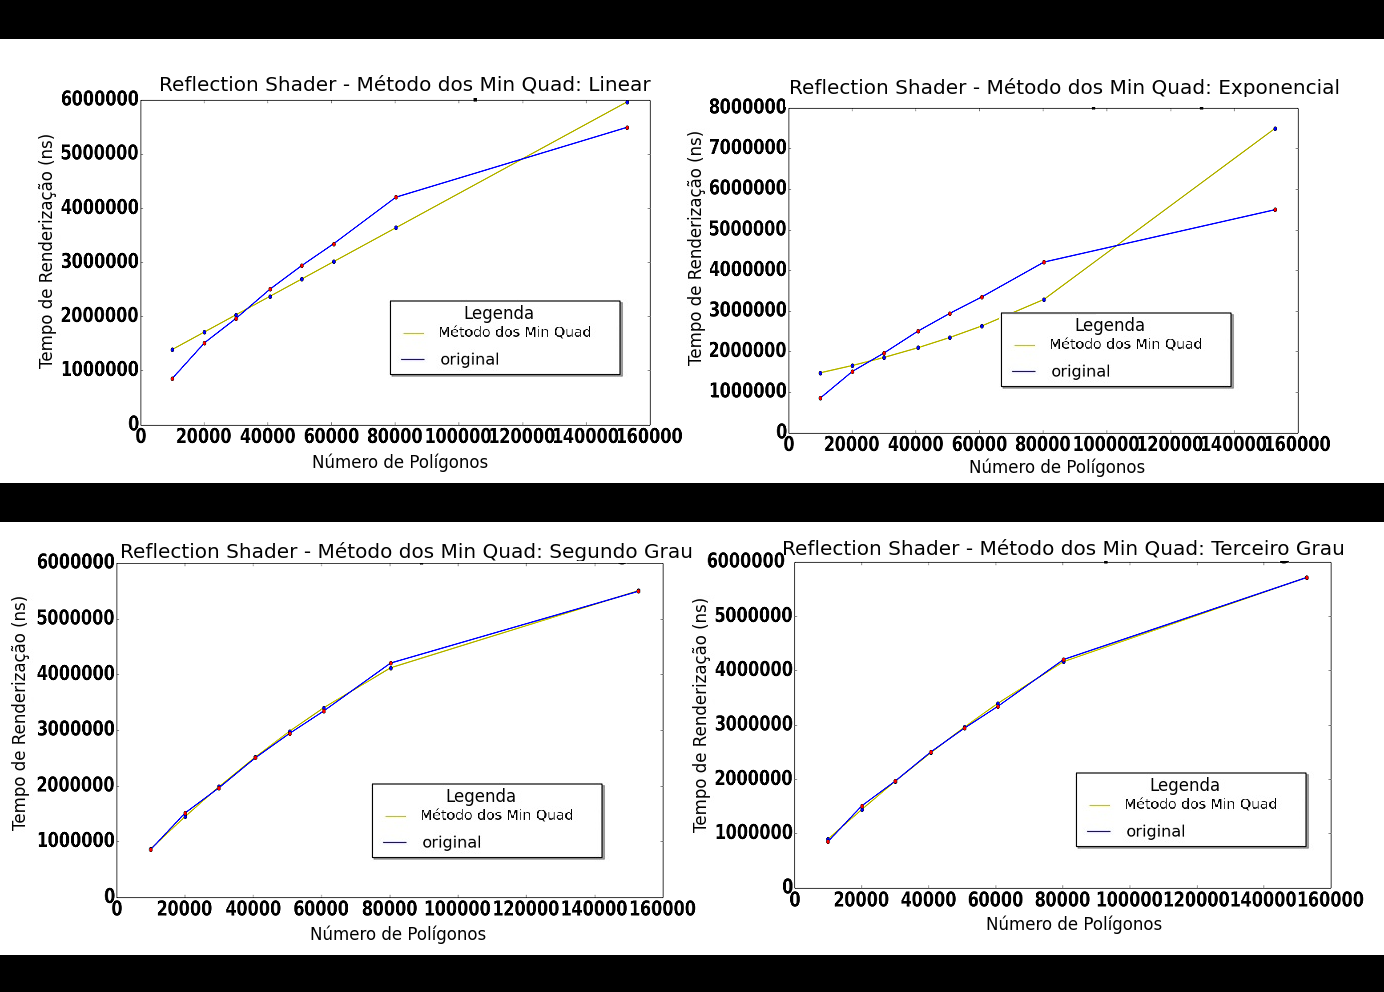
\includegraphics[keepaspectratio=true,scale=0.4]{figuras/minquad_render_time_pt.png}
	\caption{Ajustes linear, segundo, terceiro graus e exponencial do processo de renderização para o \textit{Nexus 4}}
	\label{nexus2_ajuste}
	\end{figure}	

	Com o dispositivo \textit{HTC One} foi possível apenas realizar o cálculo para o \textit{vertex} e \textit{fragment shaders}, pois ele não dá suporte à extensão da \textit{OpenGL ES} utilizada para a coleta do tempo do processo de renderização. A Figura \ref{htc1} mostra os gráficos plotados para o \textit{vertex} e \textit{fragment shaders} do \textit{Gouraud Shader} (\textit{shader} exemplo utilizado para comparação), em que os formatos são semelhantes aos obtidos com o \textit{Nexus 4}. Assim como no \textit{Nexus 4}, o \textit{vertex shader} também teve comportamento linear e para o \textit{fragment shader}, a melhor aproximação foi uma curva de terceiro grau (Figura \ref{htc1_ajuste}). 

	\begin{figure}[ht]
	\centering
		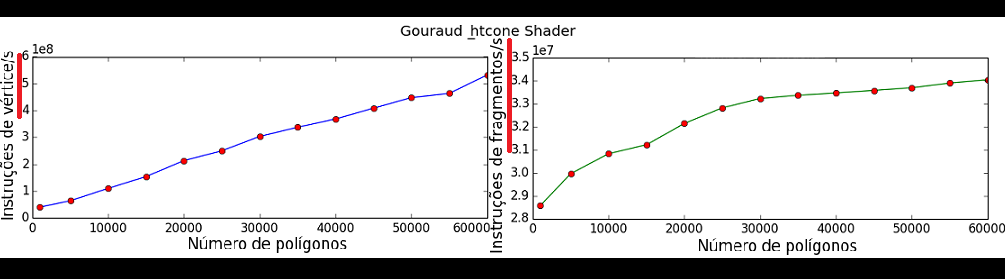
\includegraphics[keepaspectratio=true,scale=0.55]{figuras/htc_render_pt.png}
	\caption{Gráficos do \textit{Gouraud Shader} para o \textit{HTC One}}
	\label{htc1}
	\end{figure}

	\begin{figure}[ht]
	\centering
		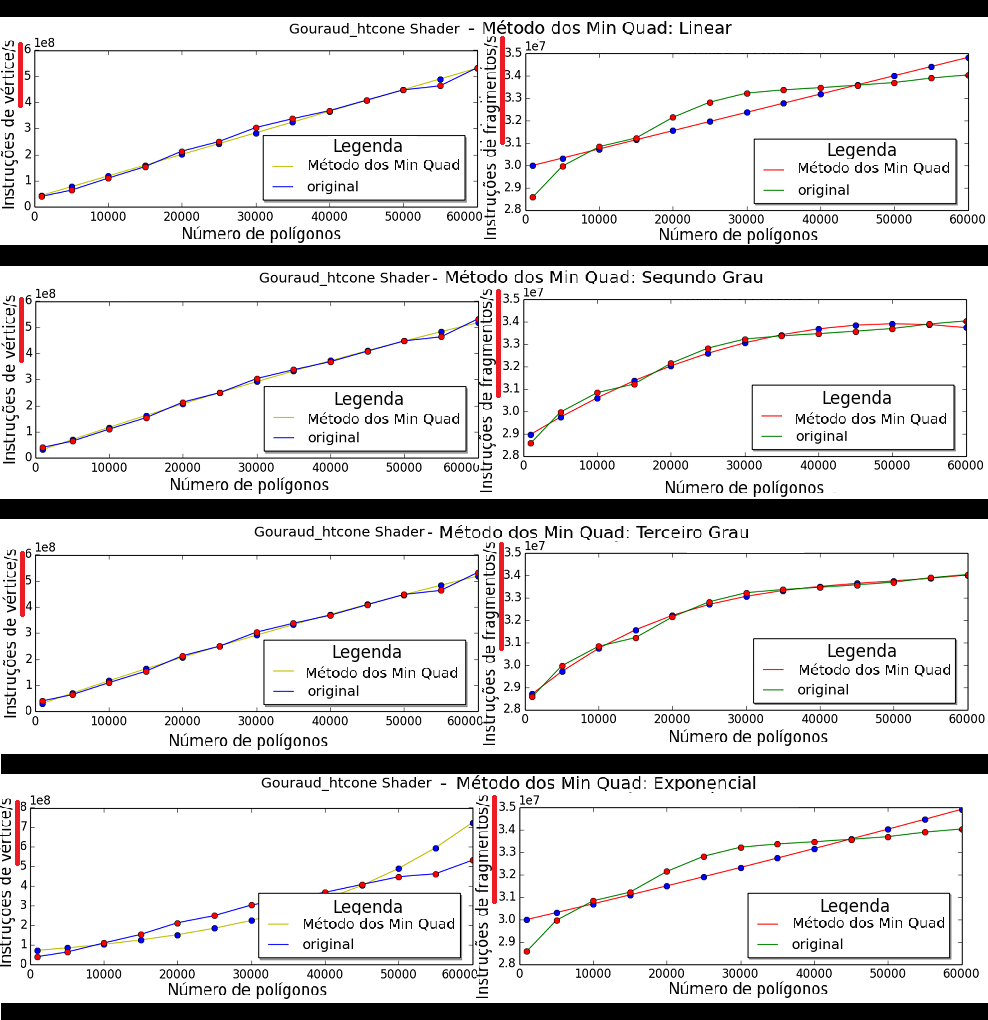
\includegraphics[keepaspectratio=true,scale=0.6]{figuras/htc_minquad_render_pt.png}
	\caption{Ajustes linear, segundo, terceiro graus e exponencial de cada tipo de \textit{shader} para o \textit{HTC One}}
	\label{htc1_ajuste}
	\end{figure}	
	
	A Figura \ref{nexus_htc} mostra as curvas dos \textit{shaders} com relação ao \textit{Nexus 4} e ao \textit{HTC One} plotadas em um mesmo gráfico.	

	\begin{figure}[ht]
	\centering
		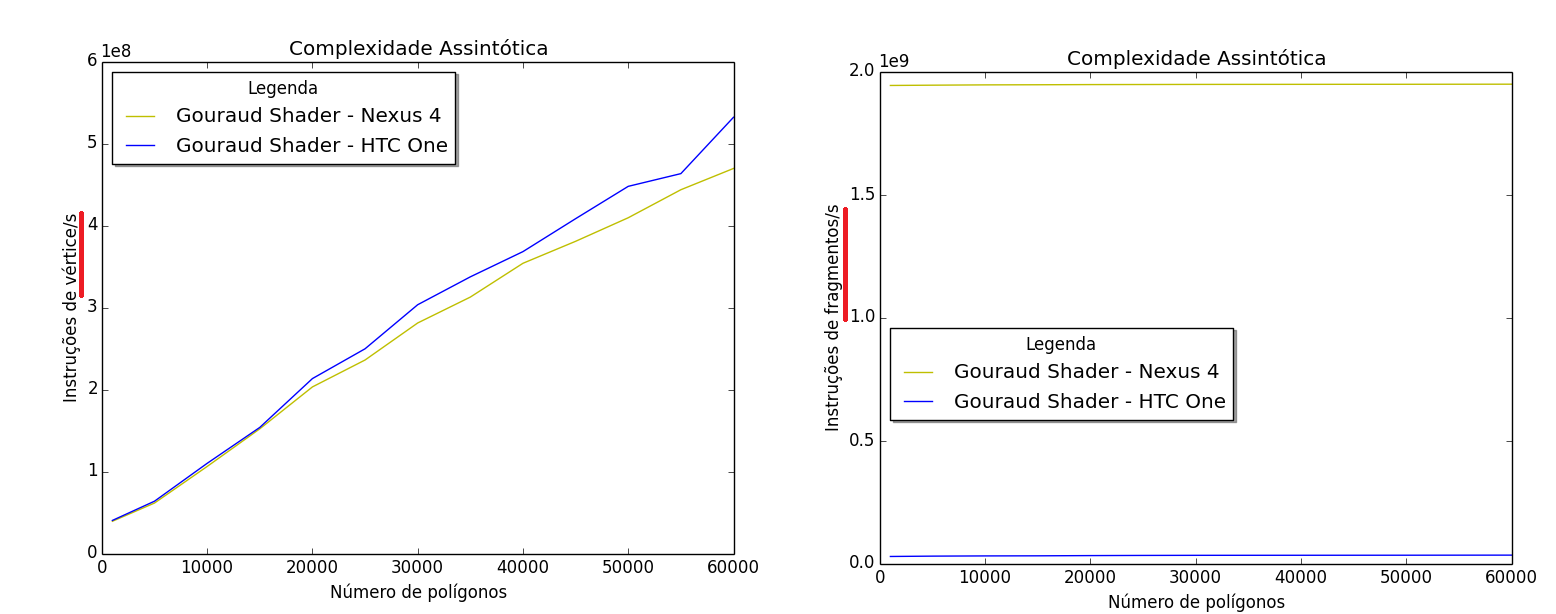
\includegraphics[keepaspectratio=true,scale=0.4]{figuras/nexus_htc.png}
	\caption{Comparação entre as curvas dos \textit{shaders}: \textit{Nexus 4} e \textit{HTC One}}
	\label{nexus_htc}
	\end{figure}	

\section{Dispositivos \textit{iOS}} 

	Para os dispositivos \textit{iPhone 5s} e \textit{iPad Air}, foi possível apenas realizar as medições quanto ao processo de renderização, pois a ferramenta utilizada não provê medições quanto ao \textit{vertex} e \textit{fragment shaders}.  A Figura \ref{ios1} mostra o gráfico plotado para o \textit{shader} tomado como exemplo de comparação, o \textit{Gouraud Shader}. O formato das curvas obtidas são semelhantes ao do \textit{Nexus 4}, e assim como ele, o melhor ajuste foi uma curva de terceiro grau (Figura \ref{ios1_ajuste}). 

	\begin{figure}[ht]
	\centering
		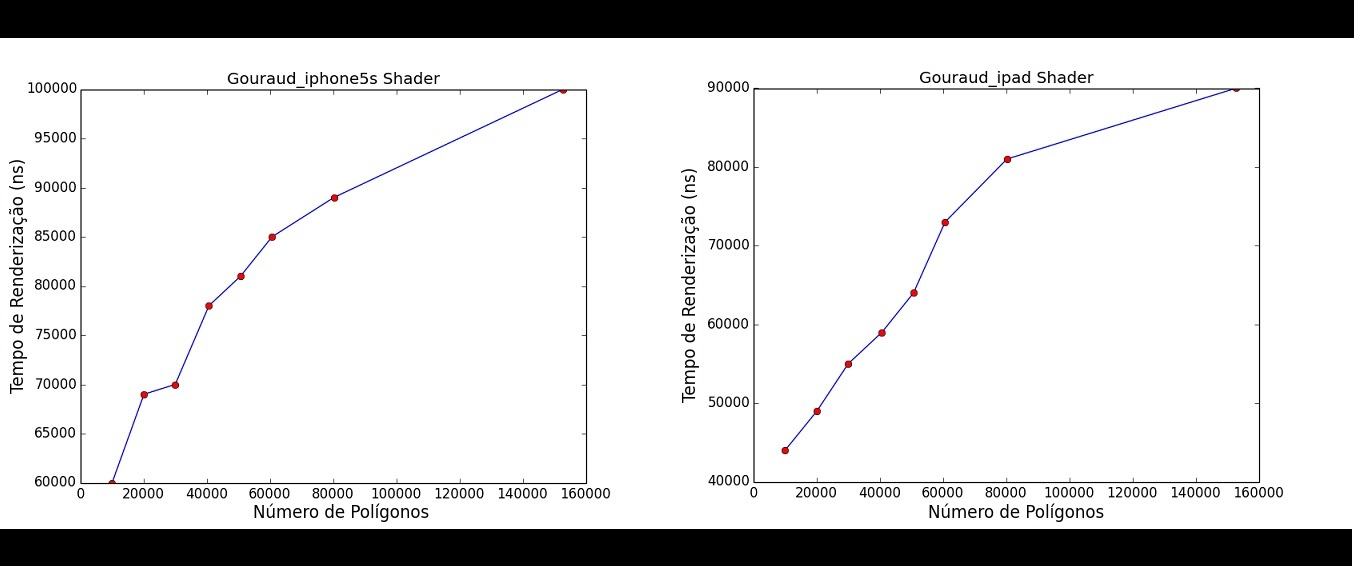
\includegraphics[keepaspectratio=true,scale=0.35]{figuras/ios_render_time_pt.jpg}
	\caption{Gráficos relacionados ao tempo de renderização em nanosegundos para os dispositivos \textit{iOS}}
	\label{ios1}
	\end{figure}	

	\begin{figure}[ht]
	\centering
		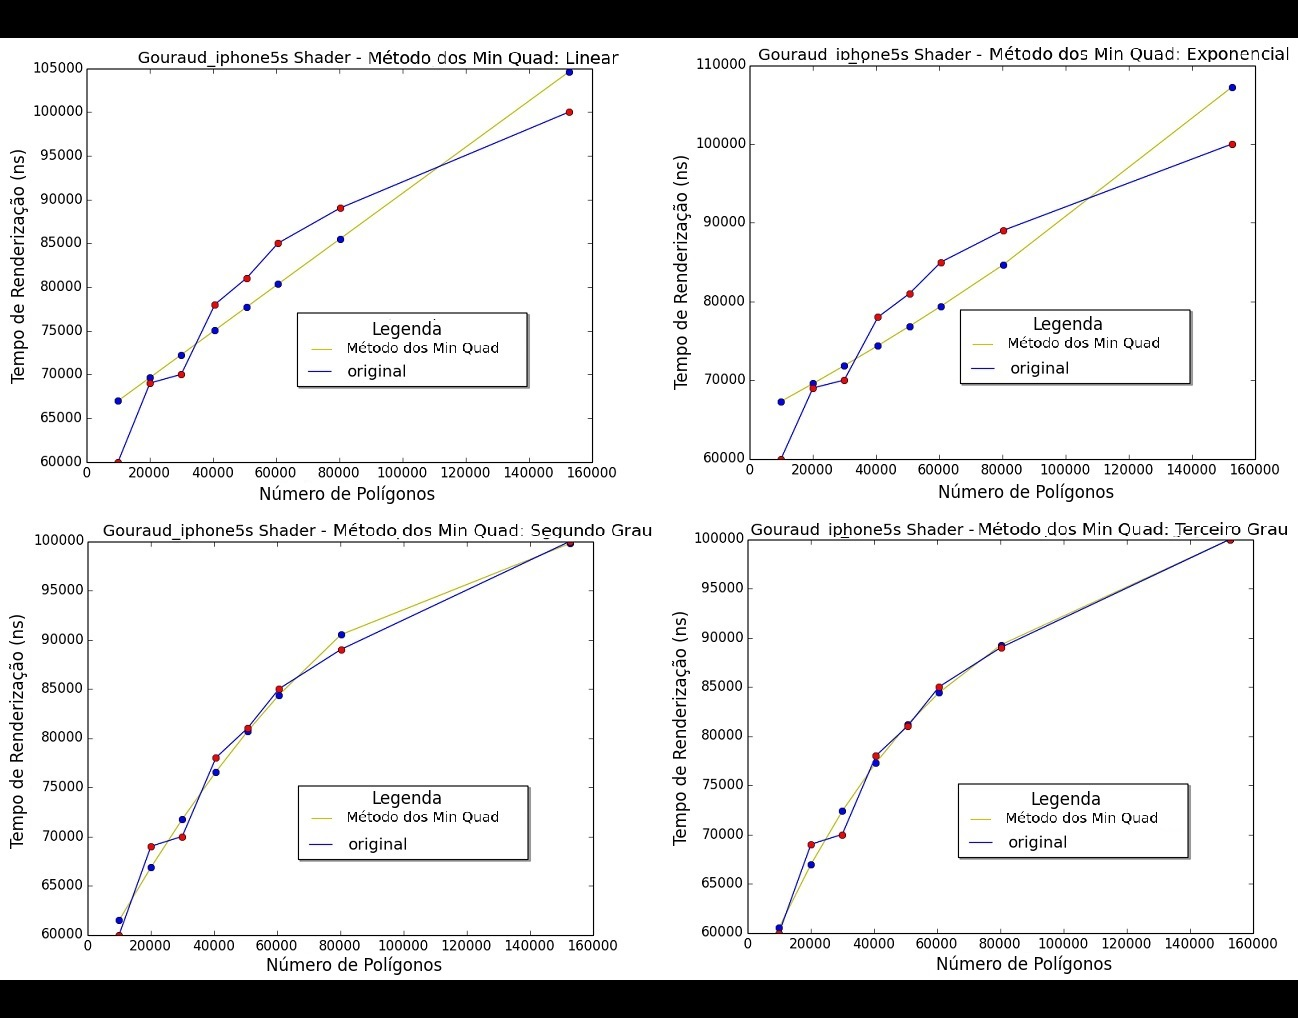
\includegraphics[keepaspectratio=true,scale=0.35]{figuras/ios_minquad_render_pt.jpg}
	\caption{Ajustes linear, segundo, terceiro graus e exponencial do processo de renderização para dispositivo \textit{iOS}}
	\label{ios1_ajuste}
	\end{figure}	

	A Figura \ref{nexus_ios} faz uma comparação entre as curvas dos \textit{shaders} com relação ao \textit{Nexus 4} e os dispositivos da plataforma \textit{iOS} que são plotadas em um mesmo gráfico.	

	\begin{figure}[ht]
	\centering
		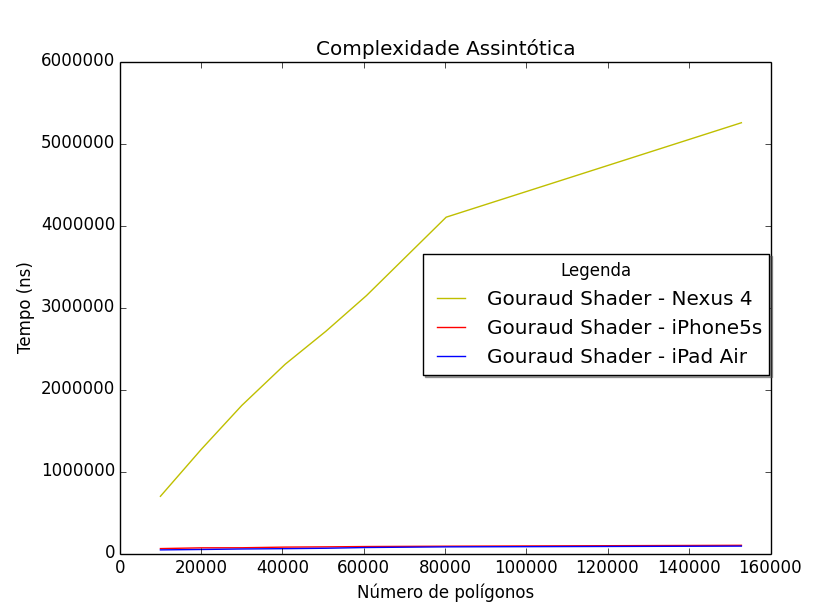
\includegraphics[keepaspectratio=true,scale=0.4]{figuras/render_time_devices.png}
	\caption{Comparação entre as curvas dos \textit{shaders}: \textit{Nexus 4}, \textit{iPhone 5s} e \textit{iPad Air}}
	\label{nexus_ios}
	\end{figure}	

\section{Análise das Equações Obtidas} 
\label{analieq}	

	As equações calculadas para cada \textit{shader} do dispositivo \textit{Nexus 4} (relacionadas ao vértice e fragmento) são mostradas na Tabela \ref{equacoes}. Embora as curvas sejam de mesma família, os seus coeficientes não são idênticos. Os \textit{shaders} relativamente mais simples tem inclinação de reta menor, assim como os coeficientes dos termos $x^2$ e $x^3$. Pela análise das equações, é possível perceber que o \textit{vertex shader} de melhor desempenho é o do \textit{Flat Shader}, que apenas determina as coordenadas $x$ e $y$, já que o $z$ é sempre zero. O de pior desempenho é o \textit{Gouraud Shader}, que faz os cálculos de luz por vértice. Já o \textit{fragment shader} de melhor desempenho é o do \textit{Red Shader}, que apenas determina que a cor do fragmento seja vermelha. O de pior desempenho foi o do \textit{Phong Shader}, que faz os cálculos de luz por fragmento.

	Outra observação que pode ser feita é quanto aos \textit{shaders Gouraud} e \textit{Phong}, pois eles realizam o mesmo cálculo, porém o primeiro faz no \textit{vertex shader} e o segundo, no \textit{fragment shader}. Pela análise das equações, o desempenho relacionado ao \textit{vertex shader} do \textit{Gouraud} é pior que a do \textit{Phong} e a relacionado ao \textit{fragment shader} é melhor.  

	Além disso, com as equações é possível estimar a quantidade de instruções por segundo por vértice ou por fragmento. Tomando como exemplo o \textit{Toon Shader}, cuja curva aproximada para o \textit{vertex shader} é  $y(t) = 10.17 \times 10^6 + 4673.96t$, o número de instruções por segundo por vértice estimado para 60000 polígonos é de $29.06 \times 10^7$. Realizando a medição com a ferramenta \textit{Adreno Profiler} foi possível perceber que este valor é próximo ao medido ($28.49 \times 10^7$).

	As equações relacionadas a todo o processo de renderização do dispositivo \textit{Nexus 4} também foram calculadas e podem ser vistas na Tabela \ref{eqrender}. Assim como no caso anterior, elas são da mesma família mas possuem coeficientes diferentes. De acordo com estas equações, o \textit{shader} de pior desempenho é o de Reflexão, que pela análise anterior, os \textit{shaders} de vértice e fragmento estavam entre os de pior desempenho. 

	Outro resultado relevante está relacionado ao \textit{Gouraud} e ao \textit{Phong Shader}, em que na análise anterior, o primeiro possui o pior desempenho entre os \textit{shaders} de vértice e o segundo, entre os \textit{shaders} de fragmento.  Mas o que possui o pior desempenho entre os dois, em relação ao processo de renderização como um todo, é o \textit{Phong shader}. Este resultado é consistente, pois o \textit{fragment shader}, pelo experimento realizado, possui complexidade assintótica $O(n^3)$ e o \textit{vertex shader}, $O(n)$, influenciando neste pior desempenho. 

	Pelo experimento realizado, os \textit{shaders} de melhores desempenhos foram o \textit{Flat}, \textit{Toon} e \textit{Red}. Além disso, utilizando as equações calculadas, a fim de estimar o tempo para 170.000 polígonos, por exemplo, essa análise se confirma, como é mostrada na Tabela \ref{estimativa}.

	\begin{table}[ht]
	\centering	
	\begin{tabularx}{0.9\textwidth}{lXX}
		\toprule
		\textbf{Nome} & \textbf{Instruções por Segundo por Vértice} & \textbf{Instruções por Segundo por Fragmento}  \\
		\midrule
		\textit{Gouraud} & $y = 40,16 \times 10^6 + 7486,43t$ & $y = 19,43 \times 10 ^8 + 297,00t - 0,0065t^2 + 0,50 \times 10^{-7}t^3 $  \\
		\textit{Phong} &  $y = 14,95 \times 10^6 + 5211,02t$ & $y = 19,84 \times 10^8 + 1752,43t - 0,0389t^2 + 3,32 \times 10^{-7}t^3$ \\
		\textit{Red} & $y = 8,02 \times 10^6 + 4545,69t$ & $y = 19,39 \times 10 ^8 + 64,34t - 0,00090t^2 + 0,05 \times 10^{-7}t^3$\\
		\textit{Toon} & $y = 10,17 \times 10^6 + 4673,96t$ & $y = 19,44 \times 10 ^8 + 268,89t - 0,0044t^2 + 0,30 \times 10^{-7}t^3$\\
		\textit{Flat} & $y = 7,65 \times 10^6 + 3738,61t$ & $y = 19,39 \times 10 ^8 + 74,94t - 0,0013t^2 + 0,08 \times 10^{-7}t^3$ \\
		\textit{Random Color} & $y = 20,58 \times 10^6 + 5640,13t$ & $y = 19,43 \times 10 ^8 + 250,33t - 0,0050t^2 + 0,37 \times 10^{-7}t^3$\\
		\textit{Simple Texture} & $y = 8,80 \times 10^6 + 4540,32t$ & $y = 19,41 \times 10 ^8 + 160,00t - 0,0030t^2 + 0,22 \times 10^{-7}t^3$\\
		\textit{CubeMap} & $y = 8,67 \times 10^6 + 4540,40t$ & $y = 19,43 \times 10 ^8 + 245,89t - 0,0047t^2 + 0,37 \times 10^{-7}t^3$ \\
		\textit{Reflection} & $y = 18,03 \times 10^6 + 5470,95t$ & $y = 19,59 \times 10 ^8 + 698,57t - 0,0094t^2 + 0,47 \times 10^{-7}t^3$ \\
	
		\bottomrule
	\end{tabularx}
	\caption{Equações relacionadas ao \textit{vertex shader} e \textit{fragment shader}}
	\label{equacoes}
	\end{table}

	\begin{table}[ht]
	\centering	
	\begin{tabularx}{0.9\textwidth}{lX}
		\toprule
		\textbf{Nome} & \textbf{Tempo do Processo de Renderização (ns)}  \\
		\midrule
		\textit{Gouraud} &  $y = 24,31 \times 10^4 + 48,89t + 7,60 \times 10^{-5}t^2 - 1,19 \times 10^{-9}t^3$\\
		\textit{Phong} &   $y = 31,25 \times 10^4 + 49,28t + 0,12 \times 10^{-5}t^2 - 1,43 \times 10^{-9}t^3$\\
		\textit{Red} & $y = 30,37 \times 10^4 + 32,92t + 0,26 \times 10^{-5}t^2 - 0.00019 \times 10^{-9}t^3$\\
		\textit{Toon} & $y = 27,28 \times 10^4 + 37,30t + 0,23 \times 10^{-5}t^2 - 1,93 \times 10^{-9}t^3$\\
		\textit{Flat} & $y = 32,82 \times 10^4 + 33,84t + 0,28 \times 10^{-5}t^2 - 2,15 \times 10^{-9}t^3$\\
		\textit{Random Color} & $y = 26,25 \times 10^4 + 38,42t + 0,20 \times 10^{-5}t^2 - 1,76 \times 10^{-9}t^3$\\
		\textit{Simple Texture} & $y = 24.51 \times 10^4 + 38,88t + 0,18 \times 10^{-5}t^2 - 1,65 \times 10^{-9}t^3$\\
		\textit{CubeMap} & $y = 29,87 \times 10^4 + 44,70t + 0,11 \times 10^{-5}t^2 - 1,28 \times 10^{-9}t^3$\\
		\textit{Reflection} & $y = 33,63 \times 10^4 + 57,31t - 9,18 \times 10^{-5}t^2 - 0,35\times 10^{-9}t^3$ \\
		
		\bottomrule
	\end{tabularx}
	\caption{Equações relacionadas ao tempo do processo de renderização}
	\label{eqrender}
	\end{table}


	\begin{table}[ht]
	\centering	
	\begin{tabularx}{0.9\textwidth}{lc}
		\toprule
		\textbf{Nome} & \textbf{Tempo do Processo de Renderização (ns)}  \\
		\midrule
		\textit{Gouraud} &  4.923.257\\
		\textit{Phong} &   5.072.434\\
		\textit{Red} & 3.825.594\\
		\textit{Toon} & 3.687.182\\
		\textit{Flat} & 3.653.955\\
		\textit{Random Color} & 3.967.677\\
		\textit{Simple Texture} & 4.065.117\\
		\textit{CubeMap} & 4.638.068\\
		\textit{Reflection} & 5.727.936\\
	
	
		\bottomrule
	\end{tabularx}
	\caption{Exemplo de estimativa para 170.000 polígonos}
	\label{estimativa}
	\end{table}


\subsection{Comparação das Equações dos Dispositivos}

	A equação do processo de renderização também foi obtida para os dispositivos \textit{iOS}, a partir de um \textit{shader} de comparação (\textit{Gouraud Shader}). A Tabela \ref{render_time_comp} mostra a comparação entre as equações destes dispositiivos e o \textit{Nexus 4}. Pelas medições realizadas e equações obtidas, foi possível perceber que o dispositivo de melhor desempenho foi o \textit{iPad Air}, que como é mostrado na Seção \ref{equip}, é o dispositivo com a melhor configuração de \textit{hardware} e o que obteve melhor posição no aplicativo de \textit{benchmarking} também mostrado nesta seção. O de pior desempenho foi o \textit{Nexus 4}, que dentre estes dispositivos é o que tem a pior configuração de \textit{hardware}.

	\begin{table}[ht]
	\centering	
	\begin{tabularx}{0.9\textwidth}{lX}
		\toprule
		\textbf{Dispositivo} & \textbf{Tempo do Processo de Renderização (ns)}  \\
		\midrule
		\textit{Nexus 4} &  $y = 24,31 \times 10^4 + 48,89t + 7,60 \times 10^{-5}t^2 - 1,19 \times 10^{-9}t^3$\\
		\textit{iPhone 5s} &   $y = 5,32 \times 10^4 + 0,79t - 0,54 \times 10^{-5}t^2 + 0,02 \times 10^{-9}t^3$\\
		\textit{iPad Air} & $y = 4,03 \times 10^4 + 0,35t + 0,44 \times 10^{-5}t^2 - 0.03 \times 10^{-9}t^3$\\	
		\bottomrule
	\end{tabularx}
	\caption{Equações do processo de renderização do \textit{Gouraud Shader}}
	\label{render_time_comp}
	\end{table}

	As equações quanto ao \textit{vertex} e \textit{fragment shaders} também foram obtidas para o dispositivo \textit{HTC One}. A Tabela \ref{vertex_frag_comp} mostra a comparação entre as equações deste dispositivo e o \textit{Nexus 4}. Pelas medições realizadas e equações obtidas, o \textit{HTC One} teve melhor desempenho com relação ao \textit{fragment shader}. Pela Seção \ref{equip} ele é um dispositivo superior ao \textit{Nexus 4} e obteve posição um pouco melhor no aplicativo de \textit{benchmarking}.  E isto é confirmado pelo resultado obtido, pois o processo de fragmento possui complexidade assintótica maior que o de vértice. 

	\begin{table}[ht]
	\centering	
	\begin{tabularx}{0.9\textwidth}{lXX}
		\toprule
		\textbf{Dispositivo} & \textbf{Instruções por Segundo por Vértice} & \textbf{Instruções por Segundo por Fragmento}  \\
		\midrule
		\textit{Nexus 4} & $y = 40,16 \times 10^6 + 7486,43t$ & $y = 19,43 \times 10 ^8 + 297,00t - 0,0065t^2 + 5,06 \times 10^{-8}t^3 $  \\
		\textit{HTC One} & $y = 357,56 \times 10^6 + 8251,00t$ & $y = 0,29 \times 10 ^8 + 279,63t - 0,0052t^2 + 3,55 \times 10^{-8}t^3 $  \\

		\bottomrule
	\end{tabularx}
	\caption{Equações do\textit{vertex} e \textit{fragment shaders} para o \textit{Gouraud Shader}}
	\label{vertex_frag_comp}
	\end{table}

\subsection{Considerações Finais das Equações}

	Por meio dos resultados, foi possível perceber que o processo de renderização como um todo, calculado por meio do tempo de renderização da GPU e pela análise dos erros quadráticos, e o processo relacionado ao \textit{fragment shader} tenderam a apresentar como complexidade assintótica um polinômio de terceiro grau para qualquer \textit{shader} (variando somente os coeficientes das funções).

	 Porém, mesmo que os erros quadráticos sejam menores para as curvas de terceiro grau (relacionadas a todo o processo de renderização e ao \textit{fragment shader}) , os coeficientes das equações mostradas na Seção \ref{analieq} para o termo $t^3$ são muito pequenos, sendo da ordem de  $10^{-7}$, $10^{-8}$ e $10^{-9}$.  No caso da ordem de $10^{-7}$, por exemplo, será somado/subtraído (de acordo com o sinal), uma unidade a cada 100 milhões de unidades de $t$ (para uma função $y(t)$), o que pode ser considerado irrelevante. Assim, neste contexto, a curva relacionada ao polinômio de segundo grau, mesmo com um erro quadrático maior, representa melhor a realidade do \textit{shader}, em que pode-se considerar a complexidade assintótica do processo de renderização e do relacionado ao \textit{fragment shader} $O(n^2)$. A Tabela \ref{equacoessec} e a Tabela \ref{eqrendersec} mostram as equações obtidas para o polinômio de segundo grau, relacionadas ao \textit{fragment shader} e a todo o processo de renderização, respectivamente, para o dispositivo \textit{Nexus 4}. As análises feitas na Seção \ref{analieq} para os polinômios de terceiro grau também se aplicam para os de segundo grau, em que o \textit{shader} de pior desempenho (relacionado ao processo do \textit{fragment shader}) é o \textit{Phong Shader}, por exemplo. 

	\begin{table}[ht]
	\centering	
	\begin{tabularx}{0.9\textwidth}{lX}
		\toprule
		\textbf{Nome} & \textbf{Instruções por Segundo por Fragmento}  \\
		\midrule
		\textit{Gouraud} & $y = 19,43 \times 10 ^8 + 187,41t - 0,0019t^2$  \\
		\textit{Phong}& $y = 19,87 \times 10^8 + 1034,36t - 0,0087t^2$ \\
		\textit{Red} & $y = 19,39 \times 10 ^8 + 53,58t - 0,00044t^2 $\\
		\textit{Toon}& $y = 19,44 \times 10 ^8 + 204,84t - 0,0017t^2 $\\
		\textit{Flat} & $y = 19,39 \times 10 ^8 + 57,12t - 0,00050t^2$ \\
		\textit{Random Color} & $y = 19,44 \times 10 ^8 + 170,31t - 0,0016t^2$\\
		\textit{Simple Texture} & $y = 19,41 \times 10 ^8 + 112,05t - 0,0010t^2$\\
		\textit{CubeMap} & $y = 19,43 \times 10 ^8 + 165,99t - 0,0014t^2$ \\
		\textit{Reflection} & $y = 19,59 \times 10 ^8 + 596,55t - 0,0051t^2$ \\
	
		\bottomrule
	\end{tabularx}
	\caption{Polinômios de segundo grau relacionados ao \textit{fragment shader}}
	\label{equacoessec}
	\end{table}

		\begin{table}[ht]
	\centering	
	\begin{tabularx}{0.9\textwidth}{lX}
		\toprule
		\textbf{Nome} & \textbf{Tempo do Processo de Renderização (ns)}  \\
		\midrule
		\textit{Gouraud} &  $y = 3,64 \times 10^4 + 64,62t - 0,00020t^2$\\
		\textit{Phong} &   $y = 6,263 \times 10^4 + 68,29t - 0,00021t^2$\\
		\textit{Red} & $y = -3,64 \times 10^4 + 58,80t - 0,00019t^2$\\
		\textit{Toon} & $y = -6,36 \times 10^4 + 62,91t - 0,00022t^2$\\
		\textit{Flat} & $y = -4,58 \times 10^4 + 62,31t - 0,00022t^2$\\
		\textit{Random Color} & $y = -4,37 \times 10^4 + 61,74t - 0,00021t^2$\\
		\textit{Simple Texture} & $y = -4,18 \times 10^4 + 61,72t - 0,00020t^2$\\
		\textit{CubeMap} & $y = 7,60 \times 10^4 + 61,64t - 0,00019t^2$\\
		\textit{Reflection} & $y = 27,57 \times 10^4 + 61,93t - 0,00017t^2$ \\
		
		\bottomrule
	\end{tabularx}
	\caption{Polinômios de segundo grau relacionados ao tempo do processo de renderização}
	\label{eqrendersec}
	\end{table}


	A Tabela \ref{render_time_compsec} e a Tabela \ref{vertex_frag_compsec} mostram as equações atualizadas para os polinômios de segundo grau para as comparações entre os dispositivos. Assim, percebe-se que os resultados das comparações feitas na Seção \ref{analieq} também continuam os mesmos, ainda que as equações tenham sido mudadas do polinômio de terceiro grau para o de segundo grau. 

	
	\begin{table}[ht]
	\centering	
	\begin{tabularx}{0.9\textwidth}{lX}
		\toprule
		\textbf{Dispositivo} & \textbf{Tempo do Processo de Renderização (ns)}  \\
		\midrule
		\textit{Nexus 4} &  $y = 3,64 \times 10^4 + 64,62t - 198,66 \times 10^{-6}t^2$\\
		\textit{iPhone 5s} &   $y = 5,57 \times 10^4 + 0,59t - 2,00 \times 10^{-6}t^2$\\
		\textit{iPad Air} & $y = 3,51 \times 10^4 + 0,75t - 2,53 \times 10^{-6}t^2$\\	
		\bottomrule
	\end{tabularx}
	\caption{Equações do processo de renderização do \textit{Gouraud Shader}}
	\label{render_time_compsec}
	\end{table}

	\begin{table}[ht]
	\centering	
	\begin{tabularx}{0.9\textwidth}{lXX}
		\toprule
		\textbf{Dispositivo} & \textbf{Instruções por Segundo por Vértice} & \textbf{Instruções por Segundo por Fragmento}  \\
		\midrule
		\textit{Nexus 4} & $y = 40,16 \times 10^6 + 7486,43t$ &$y = 19,43 \times 10 ^8 + 187,41t - 0,0019t^2$  \\
		\textit{HTC One} & $y = 357,56 \times 10^6 + 8251,00t$ & $y = 28,77 \times 10 ^6+ 202,81t - 0,0020t^2$  \\

		\bottomrule
	\end{tabularx}
	\caption{Equações do\textit{vertex} e \textit{fragment shaders} para o \textit{Gouraud Shader}}
	\label{vertex_frag_compsec}
	\end{table}

\section{Estimativas em Ambientes de Produção}

	No contexto de desenvolvimento de jogos, a unidade comumente utilizada para determinar o desempenho médio de uma aplicação é o FPS (\textit{Frames Per Second}) ou quadros por segundo, que é o número de imagens renderizadas por segundo. Assim, também é possível converter os resultados obtidos para esta unidade, por meio da Equação \ref{fps}, onde $t$ é o tempo em segundos (obtido do processo de renderização). Também é possível obter este tempo por meio da medição do número de instruções por segundo,  como mostra a Equação \ref{ips}, pois a ferramenta \textit{Adreno Profiler} também informa a quantidade de instruções para um \textit{frame}.

	\begin{equation}
		FPS = \frac{1} {t}
	\label{fps}
	\end{equation}

	\begin{equation}
		t = \frac{I_F} {I_PS}
	\label{ips}
	\end{equation}
	 onde $I_{F}$ é o número de instruções para um \textit{frame} e $I_{PS}$ é o número de instruções por segundo.
	
	Além disso, antes da conversão em \textit{frames} por segundo, somou-se à variável $t$ os tempos das outras funções da \textit{OpenGL ES} utilizadas para um \textit{frame} (que não variam com a quantidade de polígonos). Para a plataforma \textit{Android} estes tempos foram obtidos por meio da extensão da \textit{OpenGL ES} utilizada. Já na plataforma \textit{iOS}, a ferramenta \textit{Instruments} informa o tempo de cada função utilizada.
	
	Assim, a Tabela \ref{t_fps} mostra os resultados convertidos em \textit{frames} por segundo, para o \textit{shader Gouraud} utilizando o equipamento \textit{Nexus 4}, fazendo a ressalva de que esta medição não inclui outros fatores presentes num ambiente real de produção, como \textit{input} e física, por exemplo.

	\begin{table}[ht]
	\centering	
	\begin{tabularx}{0.9\textwidth}{XXXX}
		\toprule
		\textbf{Quantidade de Polígonos} & \textbf{Segundos - Renderização} & \textbf{Segundos - Outras Funções} & \textbf{FPS}  \\
		\midrule
		10.000 &  0,000698 &  0,0000140 & 1405 \\
		20.100 &  0,00127 &  0,0000140 & 779 \\
		30.000 &  0,00181 &  0,0000140 & 548 \\
		40.678 &  0,00231 &  0,0000140 & 430 \\
		50.679 &  0,00271 &  0,0000140 & 367 \\
		60.662 &  0,00315  &  0,0000140 & 316 \\
		80.256 &  0,00410  &  0,0000140 & 243 \\
	          152.840 & 0,00525 &  0,0000140 & 190 \\
		\bottomrule
	\end{tabularx}
	\caption{Estimativa de \textit{FPS}}
	\label{t_fps}
	\end{table}


\section{Processo Experimental da Estimação da Complexidade Assintótica}  

	Assim, o processo utilizado neste trabalho de estimação da complexidade algorítmica calculada de forma empírica, pode ser resumido na Figura \ref{processo}. A etapa de Implementar \textit{Shaders} pode ser feita por meio da utilização da base do projeto implementado, herdando-se da classe \textit{Shader} e implementando os métodos abstratos, como explicado na Seção \ref{imp}. A etapa Realização das Medições é feita de forma manual, dependendo do \textit{profiler} de GPU adequado para o \textit{device} utilizado. E a etapa Plotar Gráficos, Ajustar Curvas e Obter Equações pode ser feita através do \textit{script} criado para o ajuste das curvas.

	\begin{figure}[ht]
	\centering
		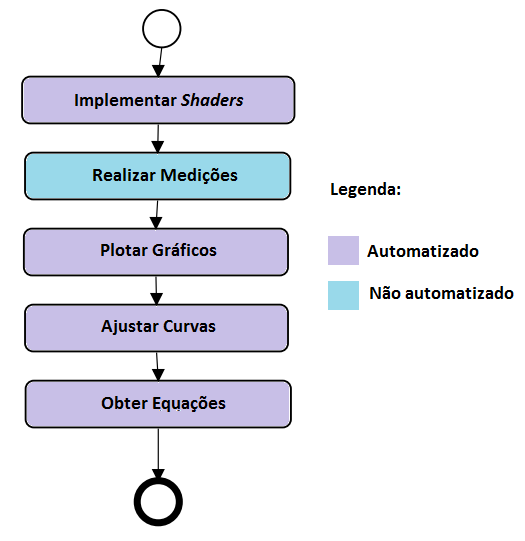
\includegraphics[keepaspectratio=true,scale=0.5]{figuras/processo.png}
	\caption{Processo da Análise de Complexidade Algorítmica.}
	\label{processo}
	\end{figure}
